\documentclass[11pt,a4paper]{article}
\usepackage[ngerman]{babel}
\usepackage[T1]{fontenc}
\usepackage[utf8]{inputenc}
\usepackage[margin=2.2cm]{geometry}
\usepackage{lmodern}
\usepackage{graphicx}
\usepackage{booktabs}
\usepackage{array}
\usepackage{fancyvrb}
\usepackage{listings}
\usepackage{xcolor}
\usepackage{float}
\usepackage{hyperref}

\lstset{basicstyle=\ttfamily\footnotesize, frame=single, columns=fullflexible,
        keywordstyle=\color{blue}\bfseries, commentstyle=\color{green!50!black}}
\lstdefinelanguage{SV}{morekeywords={module,endmodule,input,output,logic,always_comb,
        begin,end,assign}, morecomment=[l]{//}}

\title{Assignment 02 -- ALU\\\large EIT HDL -- Doku}
\author{Lukas Wolf}
\date{\today}

\begin{document}
\maketitle

\section{Aufgabe}
Das Modul \texttt{alu} verknüpft zwei 16-Bit-Werte \texttt{x} und \texttt{y}. Welche Funktion
berechnet wird, bestimmen die sechs Steuerbits \texttt{zx, nx, zy, ny, f, no}. Zusätzlich
liefert die ALU die Flags \texttt{zr} (\texttt{out == 0}) und \texttt{ng} (\texttt{out < 0}).

\section{Implementierung}
Die ALU ist in einem \texttt{always\_comb}-Block umgesetzt, Schritt für Schritt wie in der
Angabe: zuerst x und y vorbereiten, dann addieren oder UND-verknüpfen, am Ende eventuell
invertieren.

\begin{lstlisting}[language=SV]
always_comb begin
    x_zx   = zx ? '0    : x;
    x_nx   = nx ? ~x_zx : x_zx;
    y_zy   = zy ? '0    : y;
    y_ny   = ny ? ~y_zy : y_zy;
    f_out  = f  ? (x_nx + y_ny) : (x_nx & y_ny);
    no_out = no ? ~f_out : f_out;
end

assign out = no_out;
assign zr  = (out == '0);
assign ng  = out[W-1];
\end{lstlisting}

\section{Verifikation}
Die Testbench legt die 9 geforderten Operationen im Abstand von 100\,ns an und vergleicht
\texttt{out}, \texttt{zr} und \texttt{ng} mit dem erwarteten Wert. Fehler werden gezählt,
am Ende wird PASS oder FAIL ausgegeben. Gestartet wird die Simulation in ModelSim mit
\texttt{do sim\_tb\_alu.tcl}.

\paragraph{Steuerbits für \texttt{0xaa | 0x55}} (\texttt{010101}): \texttt{nx=1} und
\texttt{ny=1} invertieren x und y, \texttt{f=0} verknüpft sie mit UND, \texttt{no=1}
invertiert das Ergebnis. Nach De Morgan gilt $\overline{\overline{x} \,\&\, \overline{y}} = x \mid y$.

\subsection*{Simulator-Ausgabe}
\VerbatimInput[fontsize=\scriptsize, frame=single]{transcript.txt}

\subsection*{Wave-Fenster}
\begin{figure}[H]\centering
  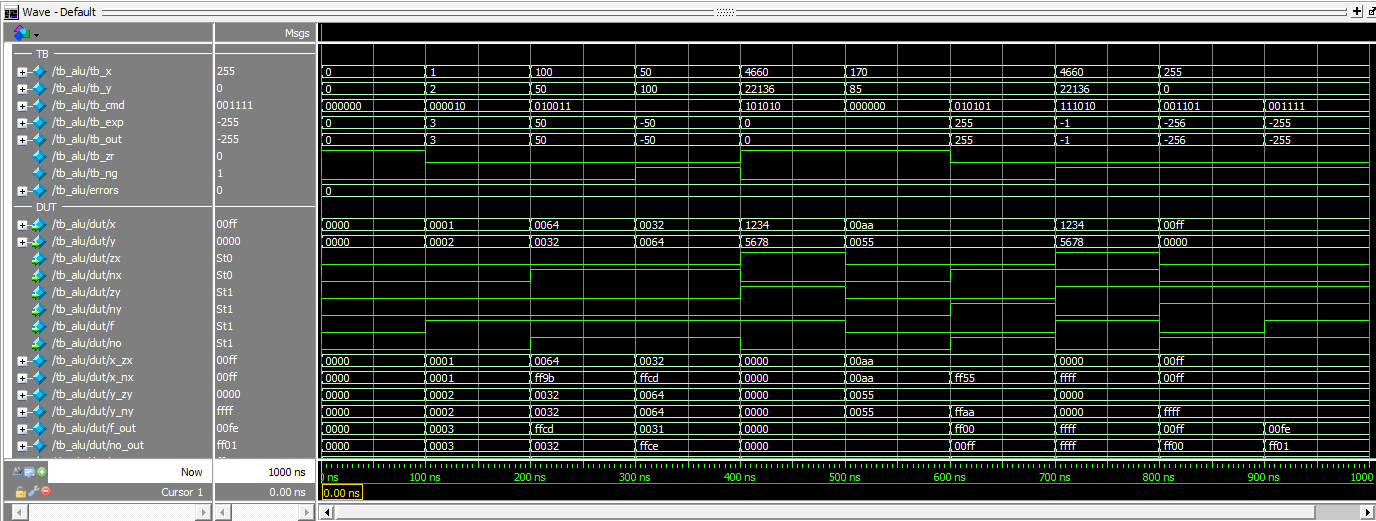
\includegraphics[width=\linewidth]{modelsim.png}
  \caption{ModelSim Wave-Fenster der Simulation von \texttt{tb\_alu}.}
\end{figure}

\paragraph{Ergebnis} Alle 9 Operationen liefern das erwartete Ergebnis, der Fehlerzähler
bleibt 0. Das Modul erfüllt damit die Spezifikation.

\section{Diskussion der Implementierungsart}
\begin{tabular}{>{\raggedright}p{3.4cm}>{\raggedright}p{5.8cm}>{\raggedright\arraybackslash}p{5.8cm}}
\toprule
Methode & Vorteile & Nachteile \\ \midrule
Gatter &
Man bestimmt jedes einzelne Gatter selbst. &
Für 16 Bit und einen Addierer sehr viel Code, fehleranfällig und schwer zu lesen. \\[1mm]
\texttt{case} über alle Funktionen &
Jede Funktion steht direkt im Code. &
Viele Zeilen, entspricht nicht dem Aufbau aus der Angabe. \\[1mm]
\textbf{\texttt{always\_comb} mit Stufen} (gewählt) &
Kurzer Code, genau wie in der Angabe aufgebaut. &
Welche Funktion berechnet wird, sieht man nur mit der Tabelle aus der Angabe. \\
\bottomrule
\end{tabular}

\end{document}
